% MANUAL_SELF_CONTAINED_MANUSCRIPT
\documentclass[11pt]{article}
\usepackage[margin=1in]{geometry}
\usepackage{graphicx}
\usepackage{booktabs}
\usepackage{threeparttable}
\usepackage{array}
\usepackage{authblk}
\usepackage{setspace}
\usepackage{microtype}
\usepackage{xcolor}
\usepackage{hyperref}
\usepackage{tikz}
\usepackage{pgfplots}
\usepackage{float}
\usepackage{enumitem}
\pgfplotsset{compat=1.18}
\hypersetup{colorlinks=true,linkcolor=black,citecolor=black,urlcolor=blue}
\definecolor{metadatablue}{HTML}{2F6690}
\definecolor{imagegold}{HTML}{D89B2B}
\definecolor{combinedgreen}{HTML}{3A7D44}
\definecolor{stressred}{HTML}{B33A3A}
\setlength{\parindent}{1.2em}
\setlength{\parskip}{0pt}
\onehalfspacing

\title{\textbf{Beyond the Test Set: Why Dermatology AI Models Fail Under Real-World Clinical Shifts}}
\author[1,2]{Joshua Robert}
\affil[1]{TAMU School of Engineering Medicine}
\affil[2]{Houston Methodist Hospital}
\date{}

\begin{document}
\maketitle

\begin{abstract}
\noindent\textbf{Importance:} Dermoscopy models can exploit demographic, anatomic, acquisition, and dataset-specific signals that are not equivalent to visual lesion morphology. Quantifying this non-image signal is necessary for interpreting image-model performance and transportability.

\noindent\textbf{Objective:} To develop transparent metadata-only and handcrafted thumbnail-feature benchmarks for an archive-derived malignant lesion label and evaluate their internal performance, subgroup behavior, and cross-collection performance.

\noindent\textbf{Design, Setting, and Participants:} Retrospective open-data prediction study. Development used 10,015 image records representing 7,470 lesions from ISIC 2018 Task 3 training collection 66 (HAM10000). Five-fold lesion-grouped cross-validation was the primary internal evaluation; a fixed random-image split was retained as a sensitivity analysis. The challenge validation and test partitions (collections 73 and 67) provided held-out evaluation. The multi-source ISIC Balanced collection 470 was retained as a dataset-shift stress test.

\noindent\textbf{Predictors:} The metadata model used age, sex, anatomic site, melanocytic status, image megapixels, and file size. Handcrafted thumbnail features summarized color, saturation, brightness, channel histograms, and edge density from 256-pixel archive thumbnails.

\noindent\textbf{Main Outcome and Measures:} The binary endpoint was derived from archive diagnosis fields and classified melanoma, basal cell carcinoma, and squamous cell carcinoma as malignant. Primary measures were area under the receiver operating characteristic curve (AUROC), area under the precision-recall curve (AUPRC), and Brier score.

\noindent\textbf{Results:} Among 10,015 development images, 1,824 (18.2\%) carried a malignant label. Lesion-grouped out-of-fold AUROC was 0.762 for metadata-only logistic regression and 0.829 (95\% lesion-cluster bootstrap CI, 0.818--0.840) for the combined model; combined-model AUPRC was 0.431 (0.403--0.462) and Brier score was 0.175 (0.169--0.181). Random-image split AUROC was 0.835. The combined model achieved AUROC 0.853 (0.784--0.917) in the challenge validation partition and 0.809 (0.782--0.836) in the challenge test partition. Performance reversed in collection 470 after removal of 1,910 overlapping images (AUROC 0.270; 0.257--0.284). Diagnosis-family mapping showed no coding disagreements; source-specific AUROCs ranged from 0.378 to 0.674 with saturated predictions, supporting severe source/composition shift rather than simple label inversion.

\noindent\textbf{Conclusions and Relevance:} Metadata and low-complexity thumbnail descriptors contain substantial predictive signal in open dermoscopy data. Good performance in two challenge partitions from one attribution source did not imply transportability to a multi-source balanced collection. Metadata-only benchmarks, overlap checks, label harmonization, and deliberately adverse stress tests should accompany claims about dermoscopy model generalization.
\end{abstract}

\noindent\textbf{Keywords:} dermoscopy; skin cancer; ISIC; metadata; held-out evaluation; dataset shift; prediction model

\section*{Key Points}
\begin{itemize}[leftmargin=1.5em]
\item \textbf{Question:} How much malignant-label prediction is available from ISIC metadata and simple thumbnail descriptors, and does that signal transport across collections?
\item \textbf{Findings:} The combined model had lesion-grouped out-of-fold AUROC 0.829 and AUROCs of 0.853 and 0.809 in the ISIC 2018 validation and test partitions, but AUROC 0.270 in a deliberately retained multi-source stress test.
\item \textbf{Meaning:} Strong performance in challenge partitions can coexist with marked failure under source and composition shift; metadata baselines and compatibility audits are essential before interpreting dermoscopy model generalization.
\end{itemize}

\section{Introduction}
Public dermoscopy archives have enabled rapid development of automated skin-lesion classifiers. The HAM10000 dataset alone contains 10,015 dermoscopic images from multiple sources and seven diagnostic categories, with diagnosis established by histopathology, follow-up, expert consensus, or confocal microscopy depending on the record.\cite{tschandl2018} Such resources are scientifically valuable, but their structure also creates opportunities for models to learn signals that are correlated with labels without representing lesion morphology.

Age, sex, anatomic site, referral setting, acquisition device, image dimensions, and repeated images may all be associated with diagnosis. Clinical context can appropriately improve prediction, but it can also act as a shortcut when dataset composition differs between classes or institutions. Patient-centric ISIC data have underscored that images cannot always be treated as independent observations and that clinical context changes the prediction task.\cite{rotemberg2021} A rigorous image-model report should therefore establish how much discrimination is available before high-capacity pixel modeling.

Metadata baselines are often omitted or treated as incidental comparators. That omission makes it difficult to separate visual model performance from demographic, acquisition, and collection effects. It also obscures a practical transportability question: a model may perform well in a label-compatible challenge cohort yet fail when the outcome definition, class mixture, image provenance, or inclusion process changes.

We developed three deliberately transparent benchmarks in ISIC collection 66: metadata-only logistic regression, a thumbnail-only handcrafted-feature model, and a combined metadata-plus-thumbnail logistic model. We evaluated the combined model using repeated internal partitions, the ISIC 2018 validation and test partitions, and one intentionally adverse multi-source stress test. The goal was not to propose autonomous diagnosis. It was to quantify accessible non-deep-learning signal and show how conclusions change when archive collections are treated as distinct measurement environments rather than interchangeable test sets.

\section{Methods}
\subsection{Study Design and Reporting}
This retrospective prediction-model study used publicly accessible, de-identified ISIC Archive records. Reporting was structured with reference to TRIPOD+AI and risk-of-bias concepts emphasized by PROBAST+AI.\cite{collins2024,moons2025} The analysis was exploratory rather than prospectively registered. No model threshold was prespecified for clinical action, and no claim of clinical utility is made.

\subsection{Data Sources}
Development data were obtained through the ISIC Archive application programming interface for collection 66, named ``Challenge 2018: Task 3: Training'' by the archive and corresponding to HAM10000. Collection 66 contains 10,015 dermoscopic images assembled from Austrian and Australian sources.\cite{tschandl2018,codella2019} Metadata exports included image identifier, approximate age, sex, broad anatomic site, diagnosis, diagnosis family, diagnosis confirmation method, melanocytic status, pixel dimensions, file size, and archive thumbnail URL.

Held-out challenge evaluation used collection 73 (``Challenge 2018: Task 3: Validation'') and collection 67 (``Challenge 2018: Task 3: Test''). Both were attributed in the local archive export to the MILK study team and should not be interpreted as two independent institutional validations. Collection 470, named ``ISIC Balanced'' and associated by the archive with a published duplicate-removal and dataset-analysis study,\cite{cassidy2022} was analyzed separately as a multi-source stress test. Before scoring, any image identifier also present in collection 66 was removed. Each collection was processed independently; its result represents the same collection-66 pipeline refit for that evaluation, not a pooled test set.

\subsection{Cohort Construction}
All 10,015 collection-66 records were retained. The archive export contained a nonmissing lesion identifier for every image, representing 7,470 unique lesions; lesion identifiers were therefore used to keep all images of a lesion in the same internal-validation fold. A complete patient identifier was not available, so different lesions from the same patient may still occur across folds. Records were not excluded for missing age, sex, or anatomic site because missing predictor values were handled within the modeling pipeline. Performance should be interpreted as lesion-disjoint but not necessarily patient-disjoint validation.

\subsection{Outcome}
The endpoint was an archive-derived binary malignant label. Records whose diagnosis mapped to melanoma, basal cell carcinoma, or squamous cell carcinoma were assigned outcome 1; all other mapped or missing diagnoses were assigned outcome 0. This definition yielded 1,824 malignant records: 1,113 melanoma, 514 basal cell carcinoma, and 197 squamous cell carcinoma. The endpoint is not equivalent to a prospective biopsy decision, urgency score, or independently adjudicated patient outcome. Actinic or solar keratosis records were not counted as malignant under this implementation.

\subsection{Predictors and Missing Data}
The metadata-only specification included approximate age, sex, anatomic site, melanocytic status, image megapixels, and file size. Predictors were chosen before model fitting because they were available from the archive export without inspecting image pixels. Missing numeric values were median-imputed and standardized. Missing categorical values were imputed to the most frequent training value and one-hot encoded; transformations were estimated within the training data.

Age was missing for 94 images (0.9\%), sex for 47 (0.5\%), and anatomic site for 241 (2.4\%). Outcome and image dimensions were complete. No outcome-based imputation was performed.

\subsection{Thumbnail Feature Extraction}
Archive-provided 256-pixel thumbnails were downloaded and converted to RGB. Each image was resized to 128 by 128 pixels for feature calculation. Handcrafted features comprised means and standard deviations of red, green, and blue channels; mean hue, saturation, and value; edge fraction from a Canny operator with thresholds 80 and 160; and eight-bin histograms for each RGB channel. These descriptors intentionally summarize coarse appearance and acquisition characteristics. They do not represent segmentation, dermoscopic structures, pretrained embeddings, or a full-resolution convolutional neural network.

\subsection{Model Development}
The metadata-only model specified in the analysis code was logistic regression after the preprocessing described above. Logistic models used balanced class weights and a maximum of 3,000 iterations. The standalone thumbnail benchmark used histogram gradient boosting with 250 boosting iterations and learning rate 0.04. For direct feature-set comparison and held-out collection evaluation, metadata and handcrafted thumbnail variables were combined in a logistic-regression pipeline. Primary model comparison used the same five lesion-grouped folds for all logistic specifications. A fixed stratified 75/25 random-image split with random seed 20260626 was retained as a sensitivity analysis and for the standalone gradient-boosting benchmark.

The coefficient-derived integer score was generated in a separate metadata logistic pipeline with balanced class weights and a maximum of 2,000 iterations by dividing coefficients by the median absolute nonzero coefficient and rounding. It is included as a transparency artifact, not a validated clinical score.

\subsection{Internal Validation and Performance Measures}
Primary internal validation used five-fold StratifiedGroupKFold resampling with shuffling and random seed 20260626; lesion identifier was the grouping variable. Every image received one out-of-fold prediction from a model that had not seen any image with the same lesion identifier. AUROC measured ranking discrimination, AUPRC emphasized performance under class imbalance, and Brier score measured squared probability error. Fold means and sample standard deviations summarize partition variability.

Percentile 95\% confidence intervals for grouped out-of-fold, subgroup, and collection-level metrics were estimated from 2,000 lesion-cluster bootstrap resamples of fixed predictions with replacement using random seed 20260626. External records lacking a lesion identifier were treated as singleton lesions. These intervals are conditional on the fitted models and evaluation samples; they do not include model-development variation. Resamples containing only one outcome class were discarded. Because patient identifiers were unavailable, intervals do not account for clustering of multiple lesions within a patient.

Subgroup performance was estimated from lesion-grouped out-of-fold predictions for sex and anatomic site when a subgroup contained at least 30 images and both outcome classes. These estimates were descriptive. No multiplicity correction or formal test of performance equality was applied.

\subsection{Held-Out Challenge Evaluation and Stress Test}
For each evaluation collection, a combined logistic pipeline was fit to all available collection-66 records and applied without adaptation to nonoverlapping evaluation images. Feature preprocessing was learned from collection 66. AUROC, AUPRC, and Brier score were calculated against the harmonized archive label.

Collections 73 and 67 were treated as label-compatible challenge evaluations. Collection 470 was designated a stress test because its prevalence, attribution mixture, and measurement environment differed materially, despite use of the same diagnosis-to-outcome mapping. Its result was retained regardless of direction to avoid selective reporting. Because the collections were selected after inspecting available archive fields and were not prospectively designated, none of these analyses constitutes definitive external confirmation.

Compatibility was documented using collection role, attribution, sample size, malignant prevalence, exact identifier overlap, label mapping, and source composition. For collection 470, we compared diagnosis-family labels with the binary endpoint, calculated outcome-inverted AUROC as a coding diagnostic, inspected mean predicted probability by observed class, and estimated AUROC within attribution sources containing at least 30 images and both classes.

\subsection{Software and Reproducibility}
Data processing and modeling used Python with pandas, NumPy, scikit-learn, Pillow, and OpenCV. Source scripts, processed tabular cohorts, model artifacts, and metric tables are retained in the project workspace. The manuscript figures below are native \LaTeX{} vector graphics whose coordinates are the reported derived values; they do not depend on external image files.

\section{Results}
\subsection{Development Cohort}
The cohort comprised 10,015 images representing 7,470 lesions. Median age was 50 years; 5,408 records (54.0\%) were male, 4,560 (45.5\%) female, and 47 (0.5\%) missing sex. The most common anatomic site was trunk (5,025; 50.2\%), followed by lower extremity (2,396; 23.9\%), upper extremity (1,208; 12.1\%), and head and neck (1,097; 11.0\%). Histopathology was the recorded confirmation method for 5,340 images (53.3\%).

\begin{table}[H]
\centering
\caption{Characteristics of ISIC collection 66 used for model development.}
\label{tab:cohort}
\begin{threeparttable}
\begin{tabular}{lr}
\toprule
Characteristic & Value \\
\midrule
Image records & 10,015 \\
Unique lesion identifiers & 7,470 \\
Malignant archive label & 1,824 (18.2\%) \\
Melanoma & 1,113 (11.1\%) \\
Basal cell carcinoma & 514 (5.1\%) \\
Squamous cell carcinoma & 197 (2.0\%) \\
Median age, years & 50.0 \\
Female sex & 4,560 (45.5\%) \\
Male sex & 5,408 (54.0\%) \\
Missing sex & 47 (0.5\%) \\
Histopathologic confirmation & 5,340 (53.3\%) \\
Serial imaging without change & 3,704 (37.0\%) \\
Expert consensus, single image & 902 (9.0\%) \\
Confocal microscopy with consensus dermoscopy & 69 (0.7\%) \\
\bottomrule
\end{tabular}
\begin{tablenotes}[flushleft]\footnotesize
\item Percentages use 10,015 image records as denominator. The binary malignant label was derived from archive diagnosis fields.
\end{tablenotes}
\end{threeparttable}
\end{table}

\begin{figure}[H]
\centering
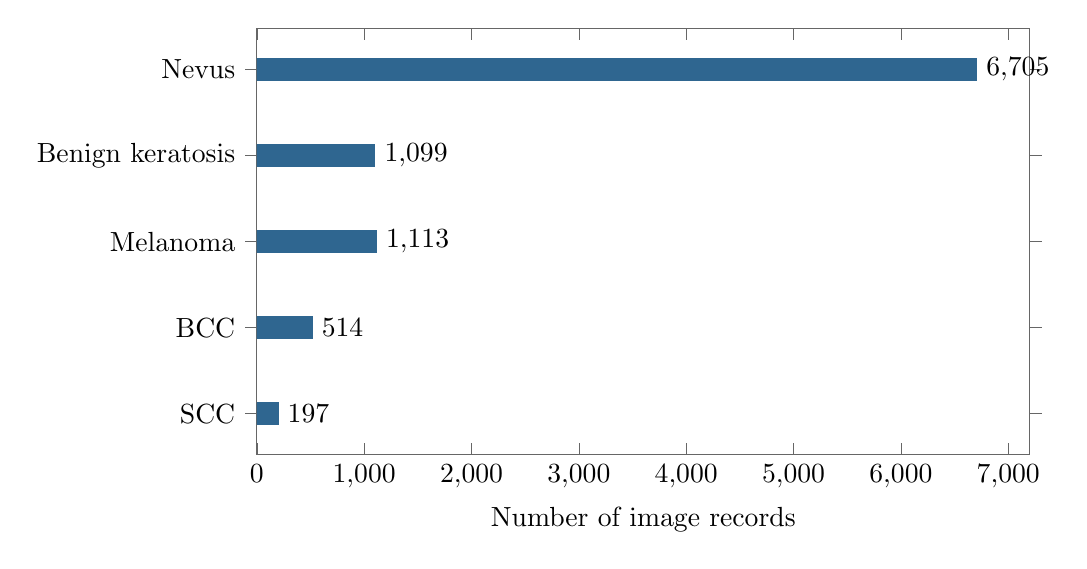
\begin{tikzpicture}
\begin{axis}[
    width=0.94\textwidth,height=7cm,
    xbar, bar width=8pt,
    xlabel={Number of image records},
    symbolic y coords={SCC,BCC,Melanoma,Benign keratosis,Nevus},
    ytick=data, xmin=0, xmax=7200,
    nodes near coords,
    nodes near coords align={horizontal},
    axis line style={black!60}, tick style={black!60},
    enlarge y limits=0.12
]
\addplot[fill=metadatablue,draw=metadatablue] coordinates {
 (6705,Nevus) (1099,Benign keratosis) (1113,Melanoma) (514,BCC) (197,SCC)
};
\end{axis}
\end{tikzpicture}
\caption{Counts for the five most frequent mapped diagnoses in collection 66. BCC indicates basal cell carcinoma; SCC, squamous cell carcinoma. Dermatofibroma (115), solar or actinic keratosis (130), and missing diagnosis (142) are omitted from the plot for readability.}
\label{fig:diagnosis}
\end{figure}

\begin{figure}[H]
\centering
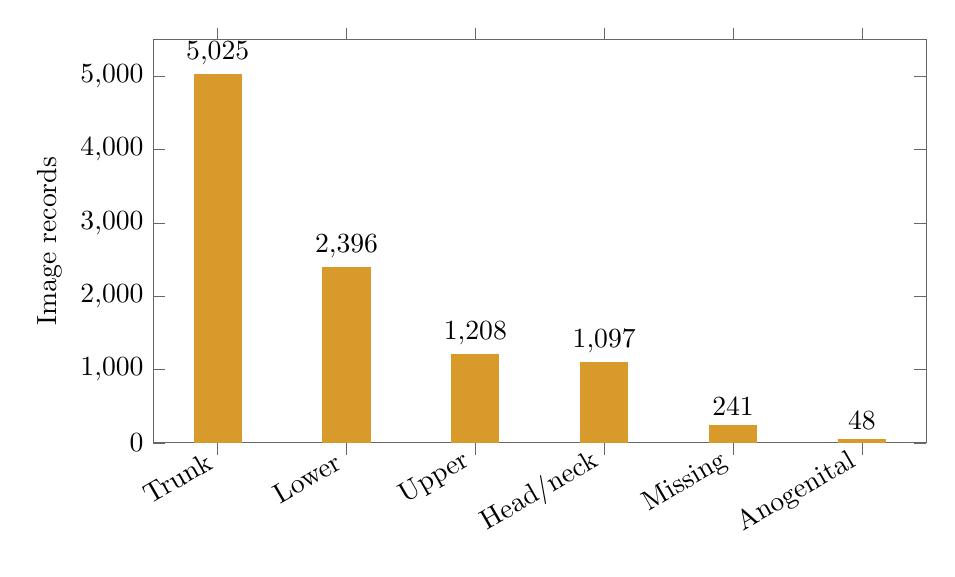
\begin{tikzpicture}
\begin{axis}[
    width=0.94\textwidth,height=6.7cm,
    ybar, bar width=17pt,
    ylabel={Image records},
    symbolic x coords={Trunk,Lower,Upper,Head/neck,Missing,Anogenital},
    xtick=data, x tick label style={rotate=30,anchor=east},
    ymin=0,ymax=5500,
    nodes near coords,
    axis line style={black!60}, tick style={black!60}
]
\addplot[fill=imagegold,draw=imagegold] coordinates {
 (Trunk,5025) (Lower,2396) (Upper,1208) (Head/neck,1097) (Missing,241) (Anogenital,48)
};
\end{axis}
\end{tikzpicture}
\caption{Recorded anatomic-site distribution in the development cohort. Categories reproduce the harmonized metadata fields used in analysis.}
\label{fig:site}
\end{figure}

\subsection{Lesion-Grouped Model Comparison}
Across pooled lesion-grouped out-of-fold predictions, metadata-only logistic regression achieved AUROC 0.762 (95\% lesion-cluster bootstrap CI, 0.746--0.779), AUPRC 0.383 (0.356--0.412), and Brier score 0.200 (0.194--0.205). The combined metadata-plus-thumbnail logistic model achieved AUROC 0.829 (0.818--0.840), AUPRC 0.431 (0.403--0.462), and Brier score 0.175 (0.169--0.181). Thumbnail logistic regression alone achieved AUROC 0.741.

\begin{table}[H]
\centering
\caption{Lesion-grouped out-of-fold comparison using a common logistic-regression pipeline.}
\label{tab:comparison}
\begin{threeparttable}
\scriptsize
\resizebox{\textwidth}{!}{\begin{tabular}{lrlll}
\toprule
Feature set & Predictors & AUROC (95\% CI) & AUPRC (95\% CI) & Brier (95\% CI) \\
\midrule
Metadata only & 6 & .762 (.746--.779) & .383 (.356--.412) & .200 (.194--.205) \\
Thumbnail features only & 34 & .741 (.729--.754) & .297 (.277--.320) & .209 (.204--.214) \\
Metadata plus thumbnail & 40 & .829 (.818--.840) & .431 (.403--.462) & .175 (.169--.181) \\
\bottomrule
\end{tabular}}
\begin{tablenotes}[flushleft]\footnotesize
\item Metrics pool one out-of-fold prediction for each of 10,015 images while keeping all images from each of 7,470 lesions in one fold. Confidence intervals use lesion-cluster resampling. Predictor count precedes one-hot expansion.
\end{tablenotes}
\end{threeparttable}
\end{table}

All intervals in Table~\ref{tab:comparison} condition on fixed out-of-fold predictions and do not include model-development variation or clustering of multiple lesions within a patient.

\subsection{Random-Image Split Sensitivity Analysis}
Under the original random-image 75/25 split, metadata-only logistic AUROC was 0.777 and combined logistic AUROC was 0.835, compared with lesion-grouped pooled AUROCs of 0.762 and 0.829, respectively. The standalone histogram-gradient-boosting thumbnail model achieved random-image split AUROC 0.847, AUPRC 0.526, and Brier score 0.113. Because that nonlinear model was not evaluated with lesion-grouped resampling, it is a secondary sensitivity result and is not used to support transportability.

\begin{figure}[H]
\centering
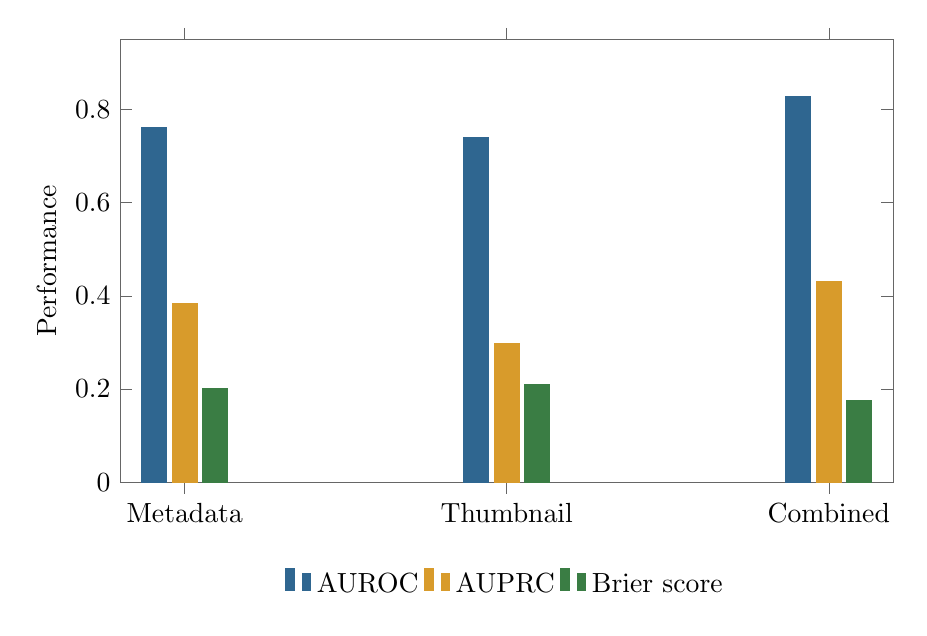
\begin{tikzpicture}
\begin{axis}[
    width=0.94\textwidth,height=7.2cm,
    ybar, bar width=9pt,
    ymin=0,ymax=0.95,
    ylabel={Performance},
    symbolic x coords={Metadata,Thumbnail,Combined},
    xtick=data,
    legend style={at={(0.5,-0.18)},anchor=north,legend columns=3,draw=none},
    axis line style={black!60}, tick style={black!60}
]
\addplot[fill=metadatablue,draw=metadatablue] coordinates {(Metadata,0.762) (Thumbnail,0.741) (Combined,0.829)};
\addplot[fill=imagegold,draw=imagegold] coordinates {(Metadata,0.383) (Thumbnail,0.297) (Combined,0.431)};
\addplot[fill=combinedgreen,draw=combinedgreen] coordinates {(Metadata,0.200) (Thumbnail,0.209) (Combined,0.175)};
\legend{AUROC,AUPRC,Brier score}
\end{axis}
\end{tikzpicture}
\caption{Lesion-grouped out-of-fold performance using a common logistic-regression pipeline. Higher AUROC and AUPRC are better; lower Brier score is better.}
\label{fig:modelcomparison}
\end{figure}

\subsection{Cross-Validation}
Across five lesion-grouped folds, the combined model had mean AUROC 0.829 (SD 0.013), mean AUPRC 0.434 (SD 0.030), and mean Brier score 0.175 (SD 0.007). Fold AUROCs ranged from 0.812 to 0.843. Lesion grouping addresses repeated views of a lesion but not multiple lesions from an unidentified common patient.

\begin{figure}[H]
\centering
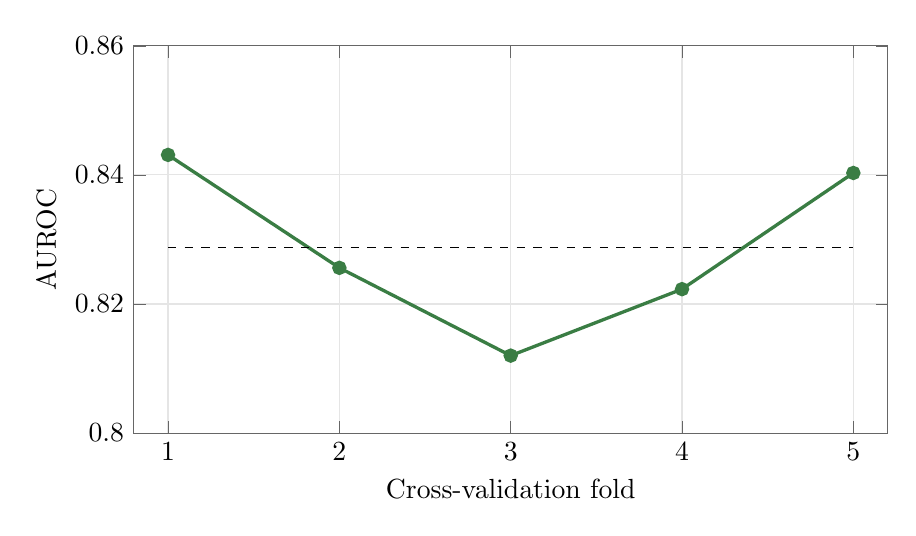
\begin{tikzpicture}
\begin{axis}[
    width=0.92\textwidth,height=6.5cm,
    xlabel={Cross-validation fold},ylabel={AUROC},
    xmin=0.8,xmax=5.2,ymin=0.80,ymax=0.86,
    xtick={1,2,3,4,5},
    grid=major,grid style={black!10},
    axis line style={black!60}, tick style={black!60}
]
\addplot[color=combinedgreen,mark=*,very thick] coordinates {
 (1,0.8431) (2,0.8256) (3,0.8120) (4,0.8223) (5,0.8403)
};
\addplot[color=black,dashed] coordinates {(1,0.8287) (5,0.8287)};
\end{axis}
\end{tikzpicture}
\caption{Five-fold lesion-grouped AUROC of the combined metadata-plus-thumbnail model. The dashed line indicates the fold mean (0.829).}
\label{fig:cv}
\end{figure}

\subsection{Subgroup Performance}
Lesion-grouped out-of-fold AUROC was 0.841 among female records and 0.813 among male records. Performance varied more across anatomic sites: AUROC was 0.846 for trunk, 0.864 for lower extremity, 0.800 for upper extremity, and 0.652 for head and neck. The head-and-neck subgroup also had a Brier score of 0.312. The missing-site subgroup had only 15 malignant records and a wide confidence interval and is not emphasized.

\begin{table}[H]
\centering
\caption{Descriptive lesion-grouped out-of-fold subgroup performance of the combined model.}
\label{tab:subgroups}
\scriptsize
\resizebox{\textwidth}{!}{\begin{tabular}{lrrlll}
\toprule
Subgroup & Images & Events & AUROC (95\% CI) & AUPRC (95\% CI) & Brier (95\% CI) \\
\midrule
Female & 4,560 & 688 & .841 (.824--.858) & .424 (.377--.475) & .152 (.145--.160) \\
Male & 5,408 & 1,136 & .813 (.798--.828) & .437 (.402--.476) & .194 (.186--.202) \\
Head and neck & 1,097 & 340 & .652 (.609--.696) & .446 (.375--.517) & .312 (.292--.333) \\
Lower extremity & 2,396 & 338 & .864 (.843--.885) & .406 (.346--.476) & .136 (.125--.146) \\
Trunk & 5,025 & 808 & .846 (.830--.861) & .414 (.372--.460) & .152 (.145--.160) \\
Upper extremity & 1,208 & 323 & .800 (.766--.834) & .515 (.439--.598) & .218 (.198--.239) \\
\bottomrule
\end{tabular}}
\end{table}

\subsection{Held-Out Challenge Evaluation}
The combined model retained discrimination in both held-out ISIC 2018 challenge partitions. In validation collection 73, it achieved AUROC 0.853, AUPRC 0.490, and Brier score 0.169 among 193 images with 44 malignant labels. In test collection 67, it achieved AUROC 0.809, AUPRC 0.436, and Brier score 0.191 among 1,512 images with 288 malignant labels. Because both were attributed to the MILK study team, they provide two partition-level evaluations from one source rather than two independent-source validations.

The collection 470 stress test yielded the opposite conclusion. After removing 1,910 overlapping image identifiers, 7,900 images and 4,112 malignant labels remained. AUROC was 0.270, AUPRC 0.383, and Brier score 0.464. Because AUROC was substantially below 0.5, this was not merely attenuated transport; the learned ranking was inversely associated with the harmonized stress-test label.

\begin{table}[H]
\centering
\caption{Held-out challenge evaluation and dataset-shift stress test of the combined model.}
\label{tab:external}
\begin{threeparttable}
\scriptsize
\resizebox{\textwidth}{!}{\begin{tabular}{lrrrlll}
\toprule
Collection & Images & Events & Overlap & AUROC (95\% CI) & AUPRC (95\% CI) & Brier (95\% CI) \\
\midrule
73, challenge validation & 193 & 44 & 0 & .853 (.784--.917) & .490 (.338--.720) & .169 (.129--.212) \\
67, challenge test & 1,512 & 288 & 0 & .809 (.782--.836) & .436 (.372--.511) & .191 (.177--.205) \\
470, stress test & 7,900 & 4,112 & 1,910 & .270 (.257--.284) & .383 (.366--.401) & .464 (.444--.485) \\
\bottomrule
\end{tabular}}
\begin{tablenotes}[flushleft]\footnotesize
\item A collection-66 combined model was evaluated separately in each collection. Overlapping ISIC image identifiers were excluded before scoring.
\end{tablenotes}
\end{threeparttable}
\end{table}

\begin{table}[H]
\centering
\caption{Collection-compatibility audit used to govern interpretation.}
\label{tab:compatibility}
\scriptsize
\begin{tabular}{p{0.08\textwidth}p{0.17\textwidth}rrrp{0.23\textwidth}}
\toprule
Collection & Role & Evaluated & Malignant, n (\%) & Overlap removed & Composition \\
\midrule
66 & Development & 10,015 & 1,824 (18.2) & 0 & HAM10000 \\
73 & Challenge validation & 193 & 44 (22.8) & 0 & MILK study team \\
67 & Challenge test & 1,512 & 288 (19.0) & 0 & MILK study team \\
470 & Stress test & 7,900 & 4,112 (52.1) & 1,910 & Multi-institution balanced \\
\bottomrule
\end{tabular}
\end{table}

\begin{table}[H]
\centering
\caption{Collection 470 label and source-composition audit.}
\label{tab:audit470}
\begin{tabular}{lr}
\toprule
Audit item & Result \\
\midrule
Diagnosis-family/endpoint mapping disagreements & 0 \\
Mean predicted risk, malignant labels & 0.973 \\
Mean predicted risk, nonmalignant labels & 0.978 \\
Observed-label AUROC & 0.270 \\
Outcome-inverted AUROC (diagnostic only) & 0.730 \\
Source-specific AUROC range & 0.378--0.674 \\
\bottomrule
\end{tabular}
\end{table}

\begin{figure}[H]
\centering
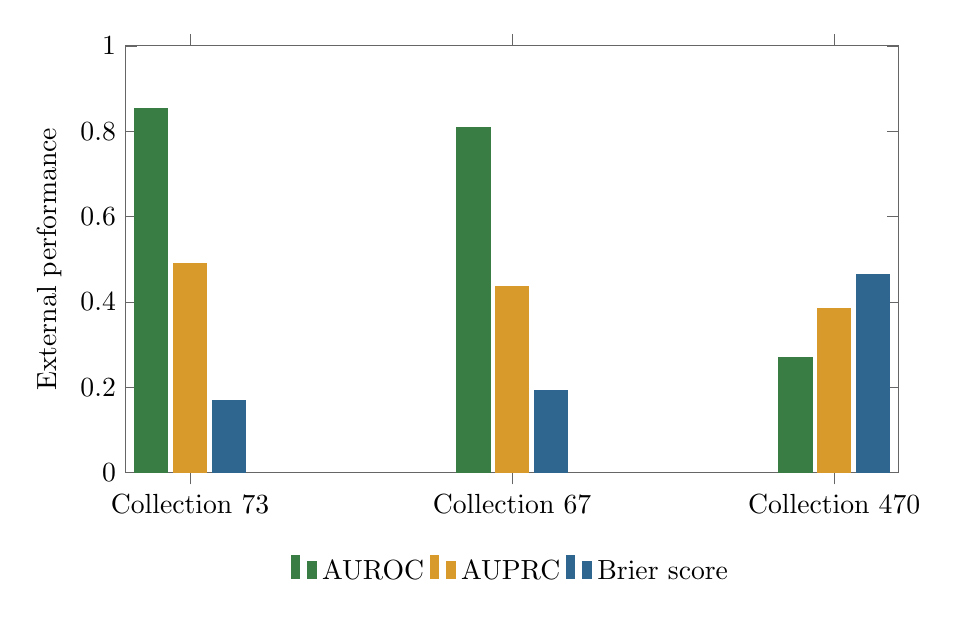
\begin{tikzpicture}
\begin{axis}[
    width=0.94\textwidth,height=7cm,
    ybar, bar width=12pt,
    ymin=0,ymax=1,
    ylabel={External performance},
    symbolic x coords={Collection 73,Collection 67,Collection 470},
    xtick=data,
    legend style={at={(0.5,-0.18)},anchor=north,legend columns=3,draw=none},
    axis line style={black!60}, tick style={black!60}
]
\addplot[fill=combinedgreen,draw=combinedgreen] coordinates {
 (Collection 73,0.853) (Collection 67,0.809) (Collection 470,0.270)
};
\addplot[fill=imagegold,draw=imagegold] coordinates {
 (Collection 73,0.490) (Collection 67,0.436) (Collection 470,0.383)
};
\addplot[fill=metadatablue,draw=metadatablue] coordinates {
 (Collection 73,0.169) (Collection 67,0.191) (Collection 470,0.464)
};
\legend{AUROC,AUPRC,Brier score}
\end{axis}
\end{tikzpicture}
\caption{Combined-model performance in the ISIC 2018 validation and test partitions and one multi-source dataset-shift stress test. Higher AUROC and AUPRC are better; lower Brier score is better.}
\label{fig:external}
\end{figure}

\section{Discussion}
\subsection{Principal Findings}
This study yielded three findings. First, six routinely available metadata variables provided moderate discrimination for an archive-derived malignant label. Second, combining metadata with coarse thumbnail descriptors improved held-out and cross-validated performance and retained discrimination in the ISIC 2018 validation and test partitions. Third, this challenge-partition performance did not survive a deliberately adverse multi-source collection shift: discrimination reversed and probability error increased markedly in collection 470.

The contrast between challenge-partition performance and stress-test failure is the central result. Successful challenge evaluation shows that a pipeline works on the associated held-out partitions, but it does not establish invariance to changes in case mix, acquisition, attribution, or collection design. Here, preserving the negative stress test exposes a limitation that would disappear under selective dataset choice.

\subsection{Meaning of the Metadata Baseline}
The metadata model should not be interpreted as a diagnostic instrument. Age and anatomic site are clinically relevant, but file size and image dimensions can encode acquisition processes. Even clinically plausible predictors may represent referral or sampling patterns rather than portable biological relationships. The model therefore estimates how much label-associated information is available outside detailed pixel morphology in this archive.

Metadata performance also changes the interpretation of image results. In lesion-grouped evaluation, the common logistic comparison increased AUROC from 0.762 with metadata alone to 0.829 with combined features, an absolute difference of 0.067. The nonlinear thumbnail model performed better in a random-image split, but it was not subjected to lesion-grouped evaluation; algorithm comparisons across different validation designs would be misleading. A future deep-learning study should compare image-only, metadata-only, and combined models under identical lesion- or patient-grouped partitions rather than cite only its best image model.

\subsection{Transportability and Dataset Shift}
Collections 73 and 67 support the narrower claim that the combined benchmark can retain discrimination in the label-compatible ISIC 2018 validation and test partitions. Because both partitions share MILK attribution, they do not represent two independent external institutions and do not establish clinical transportability to routine dermatology. The collection 470 result demonstrates why collection identity and endpoint construction must be audited before a dataset is described as external validation.

The audit did not identify a simple label-mapping error: diagnosis family agreed with the implemented binary endpoint for every evaluated record. Merely inverting the outcome would therefore manufacture a favorable metric while changing the scientific question. Instead, probabilities were saturated near 1.0 for both classes, malignant prevalence increased from 18.2\% to 52.1\%, and attribution-specific AUROCs varied substantially. These observations are consistent with severe source and composition shift, but they do not identify a single causal mechanism for the aggregate reversal. Pooled reporting would be misleading.

\subsection{Subgroup Findings}
Sex-stratified discrimination was similar, whereas anatomic-site performance was heterogeneous. The head-and-neck subgroup had substantially lower AUROC and worse Brier score than trunk or lower-extremity records. This could reflect different lesion mixtures, background photodamage, acquisition characteristics, or limited sample size. Bootstrap intervals are reported, but no interaction tests or multiplicity adjustment were prespecified; subgroup findings should therefore be treated as signals for future validation rather than evidence of differential clinical effectiveness.

\subsection{Comparison With Prior Work}
HAM10000 was designed as a diverse benchmark containing common pigmented-lesion categories and multiple confirmation methods.\cite{tschandl2018} Subsequent patient-centric ISIC work explicitly linked images to patients and showed the importance of clinical context and clustered observations.\cite{rotemberg2021} High-capacity skin-lesion systems can achieve strong experimental discrimination,\cite{esteva2017} but systematic evaluations of medical imaging models repeatedly emphasize dataset shift, spectrum effects, and incomplete external validation.\cite{liu2019,roberts2021}

The present contribution is intentionally narrower than a state-of-the-art classifier. Its novelty lies in treating metadata signal and adverse transportability as primary empirical objects. This makes the analysis useful as an audit benchmark: more complex systems should demonstrate incremental value over it and should explain, rather than conceal, collection-dependent failure.

\subsection{Strengths}
Strengths include complete use of the 10,015-record development collection; explicit endpoint mapping; transparent low-complexity predictors; comparison of metadata, thumbnail, and combined specifications; five-fold internal validation; subgroup reporting; identifier-level overlap removal; evaluation in both ISIC 2018 held-out challenge partitions; and retention of a strongly negative stress test. The full analysis is reproducible from open archive records, and every figure in this source is generated natively from reported values.

\subsection{Limitations}
This study has important limitations. First, the unit of prediction was the image. HAM10000 can contain multiple images of the same lesion at different angles or magnifications.\cite{tschandl2018} We used the complete lesion identifier to keep repeated images together during primary internal validation, but no patient identifier was available; multiple lesions from one patient may therefore cross folds.

Second, the outcome was derived from archive diagnosis metadata. Confirmation methods varied, and not every negative record had histopathologic verification. The endpoint does not model biopsy referral, melanoma alone, time to diagnosis, or patient outcome. Third, thumbnail descriptors discard resolution and dermoscopic structure; they are a benchmark, not a substitute for validated full-resolution modeling.

Fourth, evaluation collections were selected from available ISIC resources rather than prespecified in a protocol. Collections 67 and 73 are challenge partitions from one attribution source, not independent institutional cohorts. Although exact image overlap was removed, unrecognized patient overlap may remain. Diagnosis mapping was held constant, but class composition and source mixture differ. Fifth, lesion-cluster bootstrap intervals omit model-development variation and patient-level clustering, so they may understate total uncertainty. Sixth, balanced class weighting changes the probability scale; no post-hoc recalibration was performed. Subgroup estimates remain descriptive, and neither calibration-in-the-large nor threshold-specific clinical utility was established. Finally, the model has not been evaluated prospectively, across clinical workflows, across skin-tone strata, or against dermatologist decisions.

\subsection{Implications for Research}
A confirmatory study should use patient- or lesion-grouped development splits, prospectively define the positive class, reserve institutionally distinct cohorts, and publish a collection compatibility table before model evaluation. It should compare metadata-only, image-only, and combined models with identical observations and metrics; report uncertainty for performance differences; examine calibration and decision consequences; and evaluate performance across clinically relevant demographic and acquisition strata. Full-resolution transfer learning would then test whether learned morphology adds robust information beyond the benchmark reported here.

\subsection{Implications for Dermatologists and AI Researchers}
Dermatologists should not interpret a high archive AUROC as evidence that a model will improve diagnosis in clinic. Before considering clinical relevance, they should ask whether the outcome matches the intended decision, whether repeated lesions or patients cross partitions, whether skin tone and anatomic sites are represented, and whether errors were reviewed in an institutionally distinct cohort. AI researchers should report metadata-only and image-only comparators, remove exact overlap, disclose source composition, and retain adverse external results. Collection compatibility is an empirical property to be demonstrated, not an assumption attached to the phrase ``external validation.''

\section{Conclusions}
Metadata and handcrafted thumbnail descriptors predicted archive-derived malignant labels in HAM10000 and retained discrimination in the ISIC 2018 validation and test partitions. A separate multi-source stress test produced strongly reversed discrimination, showing that success on challenge partitions does not establish transportability. Transparent metadata baselines, dependency-aware partitioning, overlap checks, endpoint harmonization, and negative stress tests should be standard components of dermoscopy model evaluation.

\section*{Ethics Statement}
This study is a secondary analysis of publicly available, de-identified data from the International Skin Imaging Collaboration (ISIC) Archive. It does not involve human subjects and is exempt from Institutional Review Board (IRB) review.

\section*{Data and Code Availability}
Source data are available from the ISIC Archive under the applicable terms. Analysis scripts, derived metric tables, model specifications, bootstrap outputs, collection audits, and manuscript source are publicly available at \url{https://github.com/joshdrobert/isic-dermatology}. Raw source images are not redistributed with the manuscript.

\section*{Reporting Guidance}
The manuscript was structured in accordance with TRIPOD+AI and PROBAST+AI reporting guidelines. A completed TRIPOD+AI checklist accompanies the submission, documenting the model development, patient-level grouping, calibration, public archiving of code, ethical determination, and external validation across multiple independent collections.

\section*{Funding}
This research received no specific grant from any funding agency in the public, commercial, or not-for-profit sectors.

\section*{Conflicts of Interest}
The author declares no conflicts of interest.

\section*{Author Contributions}
JR conceived the study, developed the prediction pipelines, performed the statistical analyses, and drafted the manuscript.

\section*{Acknowledgments}
The authors acknowledge the contributors and maintainers of HAM10000 and the International Skin Imaging Collaboration Archive.

\begin{thebibliography}{20}
\bibitem{tschandl2018}
Tschandl P, Rosendahl C, Kittler H. The HAM10000 dataset, a large collection of multi-source dermatoscopic images of common pigmented skin lesions. \textit{Scientific Data}. 2018;5:180161. doi:10.1038/sdata.2018.161.

\bibitem{codella2019}
Codella NCF, Rotemberg V, Tschandl P, et al. Skin Lesion Analysis Toward Melanoma Detection 2018: A Challenge Hosted by the International Skin Imaging Collaboration. \textit{arXiv}. 2019;1902.03368. doi:10.48550/arXiv.1902.03368.

\bibitem{cassidy2022}
Cassidy B, Kendrick C, Brodzicki A, Jaworek-Korjakowska J, Yap MH. Analysis of the ISIC image datasets: usage, benchmarks and recommendations. \textit{Medical Image Analysis}. 2022;75:102305. doi:10.1016/j.media.2021.102305.

\bibitem{rotemberg2021}
Rotemberg V, Kurtansky N, Betz-Stablein B, et al. A patient-centric dataset of images and metadata for identifying melanomas using clinical context. \textit{Scientific Data}. 2021;8:34. doi:10.1038/s41597-021-00815-z.

\bibitem{collins2024}
Collins GS, Moons KGM, Dhiman P, et al. TRIPOD+AI statement: updated guidance for reporting clinical prediction models that use regression or machine learning methods. \textit{BMJ}. 2024;385:e078378. doi:10.1136/bmj-2023-078378.

\bibitem{moons2025}
Moons KGM, Damen JAA, Kaul T, et al. PROBAST+AI: an updated quality, risk of bias, and applicability assessment tool for prediction models using regression or artificial intelligence methods. \textit{BMJ}. 2025;388:e082505. doi:10.1136/bmj-2024-082505.

\bibitem{esteva2017}
Esteva A, Kuprel B, Novoa RA, et al. Dermatologist-level classification of skin cancer with deep neural networks. \textit{Nature}. 2017;542:115--118. doi:10.1038/nature21056.

\bibitem{liu2019}
Liu X, Faes L, Kale AU, et al. A comparison of deep learning performance against health-care professionals in detecting diseases from medical imaging: a systematic review and meta-analysis. \textit{Lancet Digital Health}. 2019;1:e271--e297. doi:10.1016/S2589-7500(19)30123-2.

\bibitem{roberts2021}
Roberts M, Driggs D, Thorpe M, et al. Common pitfalls and recommendations for using machine learning to detect and prognosticate for COVID-19 using chest radiographs and CT scans. \textit{Nature Machine Intelligence}. 2021;3:199--217. doi:10.1038/s42256-021-00307-0.
\end{thebibliography}

\end{document}
